% OLD
%\documentclass[11pt,compress,t,notes=noshow, aspectratio=169, xcolor=table]{beamer}
% new
\\documentclass[10pt,compress,t,notes=noshow, xcolor=table]{beamer}

% OLD
%\usepackage{../../style/lmu-lecture}
% new
% graphicx and color are loaded via lmu-lecture.sty
% maxwidth is the original width if it is less than linewidth
% otherwise use linewidth (to make sure the graphics do not exceed the margin)
% TODO: Remove once cleared to be superfluous
% \makeatletter
% \def\maxwidth{ %
%   \ifdim\Gin@nat@width>\linewidth
%     \linewidth
%   \else
%     \Gin@nat@width
%   \fi
% }
% \makeatother

% ---------------------------------%
% latex-math dependencies, do not remove:
% - mathtools
% - bm
% - siunitx
% - dsfont
% - xspace
% ---------------------------------%

%--------------------------------------------------------%
%       Language, encoding, typography
%--------------------------------------------------------%

\usepackage[english]{babel}
\usepackage[utf8]{inputenc} % Enables inputting UTF-8 symbols
% Standard AMS suite (loaded via lmu-lecture.sty)

% Font for double-stroke / blackboard letters for sets of numbers (N, R, ...)
% Distribution name is "doublestroke"
% According to https://mirror.physik.tu-berlin.de/pub/CTAN/fonts/doublestroke/dsdoc.pdf
% the "bbm" package does a similar thing and may be superfluous.
% Required for latex-math
\usepackage{dsfont}

% bbm – "Blackboard-style" cm fonts (https://www.ctan.org/pkg/bbm)
% Used to be in common.tex, loaded directly after this file
% Maybe superfluous given dsfont is loaded
% TODO: Check if really unused?
% \usepackage{bbm}

% bm – Access bold symbols in maths mode - https://ctan.org/pkg/bm
% Required for latex-math, preferred over \boldsymbol
% https://tex.stackexchange.com/questions/3238/bm-package-versus-boldsymbol
\usepackage{bm}

% pifont – Access to PostScript standard Symbol and Dingbats fonts
% Used for \newcommand{\xmark}{\ding{55}, which is never used
% aside from lecture_advml/attic/xx-automl/slides.Rnw
% \usepackage{pifont}

% Quotes (inline and display), provdes \enquote
% https://ctan.org/pkg/csquotes
\usepackage{csquotes}

% Adds arg to enumerate env, technically superseded by enumitem according
% to https://ctan.org/pkg/enumerate
% Replace with https://ctan.org/pkg/enumitem ?
% Even better: enumitem is not really compatible with beamer and breaks all sorts of things
% particularly the enumerate environment. The enumerate package also just isn't required
% from what I can tell so... don't re-add it I guess?
% \usepackage{enumerate}

% Line spacing - provides \singlespacing \doublespacing \onehalfspacing
% https://ctan.org/pkg/setspace
% \usepackage{setspace}

% mathtools – Mathematical tools to use with amsmath
% https://ctan.org/pkg/mathtools?lang=en
% latex-math dependency according to latex-math repo
\usepackage{mathtools}

% Maybe not great to use this https://tex.stackexchange.com/a/197/19093
% Use align instead -- TODO: Global search & replace to check, eqnarray is used a lot
% $ rg -f -u "\begin{eqnarray" -l | grep -v attic | awk -F '/' '{print $1}' | sort | uniq -c
%   13 lecture_advml
%   14 lecture_i2ml
%    2 lecture_iml
%   27 lecture_optimization
%   45 lecture_sl
\usepackage{eqnarray}
% For shaded regions / boxes
% Used sometimes in optim
% https://www.ctan.org/pkg/framed
\usepackage{framed}

%--------------------------------------------------------%
%       Cite button (version 2024-05)
%--------------------------------------------------------%

% Superseded by style/ref-buttons.sty, kept just in case these don't work out somehow.

% Note this requires biber to be in $PATH when running,
% telltale error in log would be e.g. Package biblatex Info: ... file 'authoryear.dbx' not found
% aside from obvious "biber: command not found" or similar.
% Tried moving this to lmu-lecture.sty but had issues I didn't quite understood,
% so it's here for now.

\usepackage{hyperref}

% Only try adding a references file if it exists, otherwise
% this would compile error when references.bib is not found
% NOTE: Bibliography packages (usebib, biblatex) are now loaded by ref-buttons.sty when needed
% This keeps all bibliography-related setup in one place

% Legacy \citelink command removed - superseded by ref-buttons.sty

%--------------------------------------------------------%
%       Displaying code and algorithms
%--------------------------------------------------------%

% Reimplements verbatim environments: https://ctan.org/pkg/verbatim
% verbatim used sed at least once in
% supervised-classification/slides-classification-tasks.tex
% Removed since code should not be put on slides anyway
% \usepackage{verbatim}

% Both used together for algorithm typesetting, see also overleaf: https://www.overleaf.com/learn/latex/Algorithms
% algorithmic env is also used, but part of the bundle:
%   "algpseudocode is part of the algorithmicx bundle, it gives you an improved version of algorithmic besides providing some other features"
% According to https://tex.stackexchange.com/questions/229355/algorithm-algorithmic-algorithmicx-algorithm2e-algpseudocode-confused
\usepackage{algorithm}
\usepackage{algpseudocode}

%--------------------------------------------------------%
%       Tables
%--------------------------------------------------------%

% multi-row table cells: https://www.namsu.de/Extra/pakete/Multirow.html
% Provides \multirow
% Used e.g. in evaluation/slides-evaluation-measures-classification.tex
\usepackage{multirow}

% colortbl: https://ctan.org/pkg/colortbl
% "The package allows rows and columns to be coloured, and even individual cells." well.
% Provides \columncolor and \rowcolor
% \rowcolor is used multiple times, e.g. in knn/slides-knn.tex
\usepackage{colortbl}

% long/multi-page tables: https://texdoc.org/serve/longtable.pdf/0
% Not used in slides
% \usepackage{longtable}

% pretty table env: https://ctan.org/pkg/booktabs
% Is used
% Defines \toprule
\usepackage{booktabs}

%--------------------------------------------------------%
%       Figures: Creating, placing, verbing
%--------------------------------------------------------%

% wrapfig - Wrapping text around figures https://de.overleaf.com/learn/latex/Wrapping_text_around_figures
% Provides wrapfigure environment -used in lecture_optimization
\usepackage{wrapfig}

% Sub figures in figures and tables
% https://ctan.org/pkg/subfig -- supersedes subfigure package
% Provides \subfigure
% \subfigure not used in slides but slides-tuning-practical.pdf errors without this pkg, error due to \captionsetup undefined
\usepackage{subfig}

% Actually it's pronounced PGF https://en.wikibooks.org/wiki/LaTeX/PGF/TikZ
\usepackage{tikz}

% No idea what/why these settings are what they are but I assume they're there on purpose
\usetikzlibrary{shapes,arrows,automata,positioning,calc,chains,trees, shadows}
\tikzset{
  %Define standard arrow tip
  >=stealth',
  %Define style for boxes
  punkt/.style={
    rectangle,
    rounded corners,
    draw=black, very thick,
    text width=6.5em,
    minimum height=2em,
    text centered},
  % Define arrow style
  pil/.style={
    ->,
    thick,
    shorten <=2pt,
    shorten >=2pt,}
}

%--------------------------------------------------------%
%       Beamer setup and custom macros & environments
%--------------------------------------------------------%

% Main sty file for beamer setup (layout, style, lecture page numbering, etc.)
% For long-term maintenance, this may me refactored into a more modular set of .sty files
\usepackage{../../style/lmu-lecture}
% Custom itemize wrappers, itemizeS, itemizeL, etc
\usepackage{../../style/customitemize}
% Custom framei environment, uses custom itemize!
\usepackage{../../style/framei}
% Custom frame2 environment, allows specifying font size for all content
\usepackage{../../style/frame2}
% Column layout macros
\usepackage{../../style/splitV}
% \image and derivatives
\usepackage{../../style/image}
% New generation of reference button macros
\usepackage{../../style/ref-buttons}

% Used regularly
\let\code=\texttt

% Not sure what/why this does
\setkeys{Gin}{width=0.9\textwidth}

% -- knitr leftovers --
% These may be used by knitr/R Markdown workflows in other lectures
\makeatletter
\def\maxwidth{ %
  \ifdim\Gin@nat@width>\linewidth
    \linewidth
  \else
    \Gin@nat@width
  \fi
}
\makeatother

% Define colors for syntax highlighting (may be used by knitr)
\definecolor{fgcolor}{rgb}{0.345, 0.345, 0.345}
\definecolor{shadecolor}{rgb}{.97, .97, .97}

% knitr code output environment
\newenvironment{knitrout}{}{}


% Can't find a reason why common.tex is not just part of this file?
% This file is included in slides and exercises

% Rarely used fontstyle for R packages, used only in 
% - forests/slides-forests-benchmark.tex
% - exercises/single-exercises/methods_l_1.Rnw
% - slides/cart/attic/slides_extra_trees.Rnw
\newcommand{\pkg}[1]{{\fontseries{b}\selectfont #1}}

% Spacing helpers, used often (mostly in exercises for \dlz)
\newcommand{\lz}{\vspace{0.5cm}} % vertical space (used often in slides)
\newcommand{\dlz}{\vspace{1cm}}  % double vertical space (used often in exercises, never in slides)
\newcommand{\oneliner}[1] % Oneliner for important statements, used e.g. in iml, algods
{\begin{block}{}\begin{center}\begin{Large}#1\end{Large}\end{center}\end{block}}

% Don't know if this is used or needed, remove?
% textcolor that works in mathmode
% https://tex.stackexchange.com/a/261480
% Used e.g. in forests/slides-forests-bagging.tex
% [...] \textcolor{blue}{\tfrac{1}{M}\sum^M_{m} [...]
% \makeatletter
% \renewcommand*{\@textcolor}[3]{%
%   \protect\leavevmode
%   \begingroup
%     \color#1{#2}#3%
%   \endgroup
% }
% \makeatother


% Defines macros and environments
% This file is included in slides and exercises

% Rarely used fontstyle for R packages, used only in 
% - forests/slides-forests-benchmark.tex
% - exercises/single-exercises/methods_l_1.Rnw
% - slides/cart/attic/slides_extra_trees.Rnw
\newcommand{\pkg}[1]{{\fontseries{b}\selectfont #1}}

% Spacing helpers, used often (mostly in exercises for \dlz)
\newcommand{\lz}{\vspace{0.5cm}} % vertical space (used often in slides)
\newcommand{\dlz}{\vspace{1cm}}  % double vertical space (used often in exercises, never in slides)
\newcommand{\oneliner}[1] % Oneliner for important statements, used e.g. in iml, algods
{\begin{block}{}\begin{center}\begin{Large}#1\end{Large}\end{center}\end{block}}

% Don't know if this is used or needed, remove?
% textcolor that works in mathmode
% https://tex.stackexchange.com/a/261480
% Used e.g. in forests/slides-forests-bagging.tex
% [...] \textcolor{blue}{\tfrac{1}{M}\sum^M_{m} [...]
% \makeatletter
% \renewcommand*{\@textcolor}[3]{%
%   \protect\leavevmode
%   \begingroup
%     \color#1{#2}#3%
%   \endgroup
% }
% \makeatother

\newcommand{\open}{}
\newcommand{\close}{}

\title{Interpretable Machine Learning}
% \author{LMU}
%\institute{\href{https://compstat-lmu.github.io/lecture_iml/}{compstat-lmu.github.io/lecture\_iml}}
\date{}

\begin{document}

% OLD
%\newcommand{\titlefigure}{figure/25-05-31_Hooker_2004_graph_fANOVA}
%\newcommand{\learninggoals}{
%\item One method for functional decomposition: Classical functional ANOVA (fANOVA)
%\item Algorithm for calculating the components in a fANOVA
%\item Variance decomposition in fANOVA
%}
%
%\lecturechapter{Functional ANOVA}
%\lecture{Interpretable Machine Learning}
% new
\titlemeta{
Functional ANOVA
}{
Interpretable Machine Learning
}{
figure/25-05-31_Hooker_2004_graph_fANOVA
}{

\item One method for functional decomposition: Classical functional ANOVA (fANOVA)
\item Algorithm for calculating the components in a fANOVA
\item Variance decomposition in fANOVA

}


\begin{frame}{Introduction and History of fANOVA}

\begin{itemize}
    \item One possible method to obtain functional decomposition
    \item Since 1940's: Developed under different names in mathematics and sensitivity analysis
    \item Since 1990's: Developed for probability distributions or statistical data
    \item Since 2000's: Applied to machine learning, subsequently alternatives developed extending applicability
    \item \textbf{Assumption}: Independent features
\end{itemize}

% @ Sobol-Hoeffding Decomposition: erstes Paper von (Sobol? Hoeffding?) in 1950, nur im Unit Cube, allererste HDMR \\

% Sobol in 90'ern

% Sensitivity analysis

% Hooker paper
    
\end{frame}

\begin{frame}{Standard fANOVA: Idea}

    \begin{itemize}
        \item Example:
        \begin{equation*}
            \fh(x_1, x_2) = 4 - 2x_1 + 0.3 e^{x_2} + |x_1|x_2
        \end{equation*}
        \pause
        \item \textbf{First idea:} Make sure higher-order terms don't contain lower-order terms \\
        \(\Rightarrow\) First compute lower-order terms, then higher-order terms. \\
        % \pause
        % \item \textbf{Question:} How to compute lower-order terms? \\
        % \(\leadsto\) First step: Use feature effect methods for main effects, here: PDP
        \pause
        \item \textbf{Second idea:} In first step, compute main effects using feature effect methods \\
        Here: PDP + more general PD-functions
        \pause
        \item \textbf{Idea for fANOVA:} PD-function $\fh_{S;PD} =$ sum of all components $g_{\tilde{S}}$ up to this order
        $$
        \fh_{S;PD}(\xv_S) \; = \; \sum_{V \subseteq S} g_{V}(\xv_V)
        $$
        \pause
        \item \textbf{Remember:} \\ Idea of PDPs or general PD-functions: Average out all other features
        \item[$\Rightarrow$] Total formula for calculating the components \(g_S\) in the fANOVA algorithm:
        % $$
        % \begin{aligned}
        \begin{multline*}
            g_{S} (\xv_S)
            \;=\; (\text{average out all features not contained in } S) \\
            \;-\; (\text{All lower-order components})
        \end{multline*}
        % \end{aligned}
        % $$
    \end{itemize}

    % \textbf{Idea:} Main effects via feature effect methods, here: PDP\\
    % Starting with the main effects: % One can use one of the global feature effect plots, since they exactly provide a function only depending on one feature, which models the effect of this feature on \(\fh\).
    % \textit{Link to PDP??} \\
    
    % $g_{S'}$
    % \(\Rightarrow\) fANOVA uses the same idea as PDPs, but also for higher-order terms: the resp. feature is fixed and all other features are simply averaged out. \\
    
\end{frame}

\begin{frame}{Formal Definition and Computation
% OLD
%\citebutton{Hooker (2004)}{https://dl.acm.org/doi/10.1145/1014052.1014122}
% new
\furtherreading{Hooker_2004}
}

% Components are recursively defined using marginals (here $-S = \{1, \ldots, p \} \setminus S$ denotes the set of all indizes not contained in \(S\)):
\begin{definition}
    Recursive computation using PD-functions \\
    (here $-S = \{1, \ldots, p \} \setminus S$ denotes all indices not contained in \(S\)):
    \begin{align*}
    g_{S}(\xv_S)
        & = \fh_{S;PD}(\xv_S) - \sum_{V \subsetneqq S} g_V(\xv_V)
        % = \mathbb{E}_{\Xv_{-S}} \left[\fh(\xv_S, \Xv_{-S}) \; \middle\vert \; \xv_S \right] - \sum_{V \subsetneqq S} g_V(\xv_V)
        = \mathbb{E}_{\Xv_{-S}} \left[ \; \fh(\xv_S, \Xv_{-S}) \; \right] - \sum_{V \subsetneqq S} g_V(\xv_V) \\
        & = \int \fh(\xv_S, \xv_{-S}) d \mathbb{P}(\xv_{-S}) - \sum_{V \subsetneqq S} g_V(\xv_V)
    \end{align*}
\end{definition}

\begin{itemize}
    \item Expectation integrates $\fh(\xv)$ over all input features except $\xv_S$
    % \item Subtract all components $g_V$ with $V \subsetneqq S$ to remove all lower-order effects and center the effect
    \item Subtract sum of $g_V$ to remove all lower-order effects and center the effect
    \item \textbf{Note:} If no distribution given: Uniform distribution or plain integral
\end{itemize}

\end{frame}

\begin{frame}{Formal Definition and Computation
% OLD
%\citebutton{Hooker (2004)}{https://dl.acm.org/doi/10.1145/1014052.1014122}
% new
\furtherreading{Hooker_2004}
}

% Components are recursively defined using marginals (here $-S = \{1, \ldots, p \} \setminus S$ denotes the set of all indizes not contained in \(S\)):
\begin{definition}
    Recursive computation using PD-functions \\
    (here $-S = \{1, \ldots, p \} \setminus S$ denotes all indices not contained in \(S\)):
    \begin{align*}
    g_{S}(\xv_S)
        & = \fh_{S;PD}(\xv_S) - \sum_{V \subsetneqq S} g_V(\xv_V)
        % = \mathbb{E}_{\Xv_{-S}} \left[\fh(\xv_S, \Xv_{-S}) \; \middle\vert \; \xv_S \right] - \sum_{V \subsetneqq S} g_V(\xv_V)
        = \mathbb{E}_{\Xv_{-S}} \left[ \; \fh(\xv_S, \Xv_{-S}) \; \right] - \sum_{V \subsetneqq S} g_V(\xv_V)
    \end{align*}
\end{definition}

\begin{itemize}
    % \pause
    \item Recursive computation:
    \begin{align*}
        g_{\open \emptyset \close} &= \mathbb{E}_\Xv\left[\fh(\Xv)\right] \\
        g_{\open j \close}(x_j) &= \mathbb{E}_{\Xv_{-j}}\left[\fh(\Xv) \; \vert  \; X_j = x_j \right] - g_{\open \emptyset \close}, \; \forall j \in \{1, \ldots, p\} \\% \text{ and } g_{\open 2 \close}(x_2) = \mathbb{E}_{X_{-2}}\left[\fh(\xv) \; \vert  \; x_2 \right] - g_{\open \emptyset \close}  \\
        %g_{\open 2 \close}(x_2) &= \mathbb{E}_{X_{-2}}\left[\fh(\xv) \; \vert  \; x_2 \right] - g_{\open \emptyset \close} \\
        % g_{\open j, k \close}(x_j, x_k)
        % &= \mathbb{E}_{X_{-\{ j,k \}}}\left[\fh(\xv) \; \vert \; x_j, x_k \right] - g_{\open k \close}(x_k) - g_{\open j \close}(x_j) - g_{\open \emptyset \close}, \; \forall j < k\\%,  \text{ etc.}\\
        & \vdots \\
        g_{\open 1, \dots, p \close}(\xv)
        & = \fh(\xv) -
        \textstyle\sum_{S \subsetneqq \{1,\ldots,p\}} g_{S}(\xv_S) \\
        & = \fh(\xv) -
        %\textstyle\sum_{S \subsetneqq \{1,\ldots,p\}} g_{S}(\xv_S) 
        g_{\open 1, \dots, p-1 \close}(x_{1}, \dots x_{p-1}) - \dots - g_{\open 1, 2 \close}(x_1, x_2) \\
        %&\phantom{{}={}} 
        & \quad - g_{\open p \close}(x_p)  - \dots - g_{\open 2 \close}(x_2) - g_{\open 1 \close}(x_1) - g_{\open \emptyset \close}
    \end{align*}

\end{itemize}
        
\end{frame}

\begin{frame}{Standard fANOVA -- Example}
\textbf{Example:} $\fh(\xv) = 2 + x_1^2 - x_2^2 + x_1 \cdot x_2$ (e.g., for $x_1 = 5$ and $x_2 = 10$ we have $\fh(\xv) = -23$)

\begin{itemize}
    \item Computation of components using feature values $x_1 = x_2 = (-10, -9, \ldots, 10)^\top$ gives:
    \begin{columns}[c, totalwidth=\linewidth]
    \begin{column}{0.75\textwidth}
        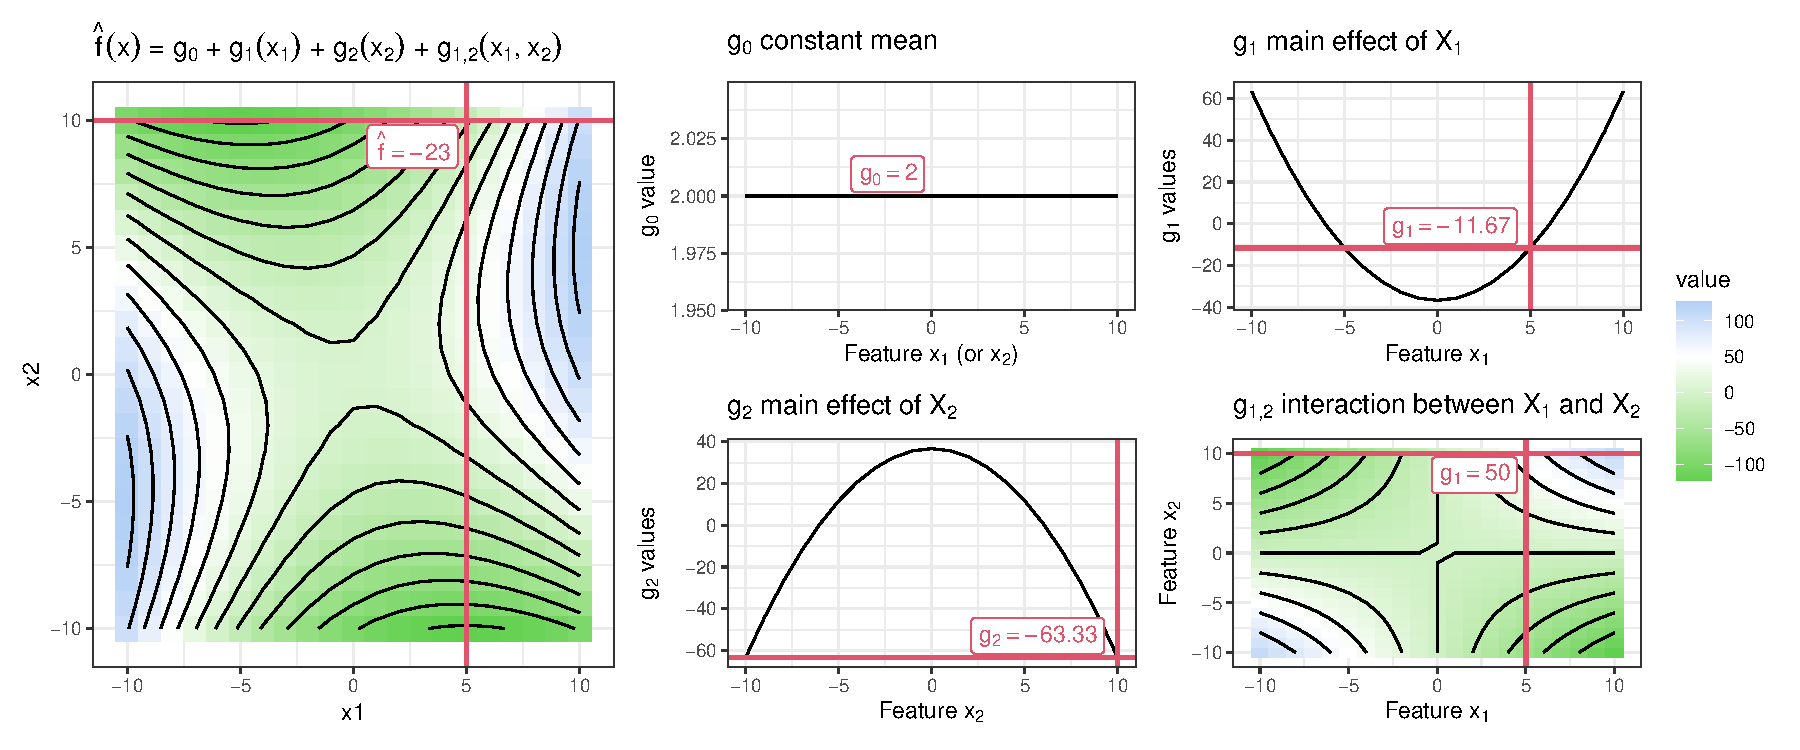
\includegraphics[width = \textwidth]{figure/decomposition}
    \end{column}
    \begin{column}{0.25\textwidth}
    For $x_1 = 5$ and $x_2 = 10$:\\
    \begin{itemize}
        \item $g_{\open \emptyset \close} = 2$
        \item $g_{\open 1 \close}(x_1) = -9.67$
        \item $g_{\open 2 \close}(x_2) = -65.33$
        \item $g_{\open 1,2 \close}(x_1, x_2) = 50$
        \item[$\Rightarrow$] $\fh(\xv) = -23$
    \end{itemize}
    \end{column}
    \end{columns}
% \pause
%     \item Vanishing condition means:
%     \begin{itemize}
%         \item $g_1$ and $g_2$ are mean-centered w.r.t. marginal distribution of $x_1$ and $x_2$
%         \item Integral of $g_{1,2}$ over marginal distribution $x_1$ (or $x_2$) is always 0.
%         %, i.e., for each slice at $x_1$ (and $x_2$), the integral of $g_{1,2}$ 
%     \end{itemize}
\end{itemize} 
\end{frame}

\begin{frame}{Standard fANOVA - Example}

\textit{In-class task}

%     [calculate a full complete example] \\

%     Analytic examples from Sobol (1993), Sobol (2001) or Hooker(2004))

%     [several examples needed, can also include those from beginning]
    
%     [problem with examples from beginning: If using fANOVA, we do not get the original components out of it again, right?]

%     -> exactly that is the case, explain the reason here: some averaged part of interaction term is moved into lower order, we need this in fANOVA, because we need a data-driven / formula-agnostic way of computing the components

%     -> use the in-class calculation task here to illustrate this
    
\end{frame}

\begin{frame}{Standard fANOVA - Example revisited}

\begin{example}

    % $$
    % \fh(x_1, x_2) = x_1^2 + \sin(\pi x_1) \cos(\pi x_2)
    % \qquad (x_1, x_2) \in [0,2]^2,
    % $$

    % Use fANOVA algorithm on example from the beginning:
    
    $$
        \fh(x_1, x_2) = 4 - 2x_1 + 0.3 e^{x_2} + |x_1|x_2 \qquad (x_1, x_2) \in [0,1]^2 \qquad \text{uniformly distributed}
    $$
    
    \begin{itemize}
        \item
        \only<1>{
        \textbf{Intercept:}
        \begin{align*}
        g_\emptyset
        &= \mathbb{E} \Bigl[ \fh(x_1, x_2) \Bigr]
        = \int_0^1 \! \int_0^1 4 - 2x_1 + 0.3 e^{x_2} + |x_1|x_2 \,dx_1\,dx_2 \\
        &= 4
            - \Bigl( \int_0^1 2x_1 \,dx_1 \Bigr)
            + \Bigl( \int_0^1 0.3 e^{x_2} \,dx_2 \Bigr)
            + \Bigl( \int_0^1 |x_1| \,dx_1 \Bigr) \Bigl( \int_0^1 x_2 \,dx_2 \Bigr) \\
        &= 4
            - 1
            + 0.3 (e - 1)
            + 0.5^2
        = 2.95 + 0.3 e.
        \end{align*}
        }
        \only<2>{
        \textbf{First-order components:}
        \begin{align*}
        g_{1}(x_1)
        &= \fh_{1;PD}(x_1) - g_\emptyset 
        = \Bigl( \int_0^1 4 - 2x_1 + 0.3 e^{x_2} + |x_1|x_2 \,dx_2 \Bigr) - g_\emptyset \\
        &= 4 - 2x_1 + 0.3 (e-1) + |x_1| \cdot \frac{1}{2} - (2.95 + 0.3e) \\
        &= -2x_1 + 0.5|x_1| + 0.75 \\
        % \end{align*}
        % }
        % \only<2>{
        % \textbf{First-order components:}
        % \begin{align*}
        g_{2}(x_2)
        &= \fh_{2;PD}(x_2) - g_\emptyset 
        = \Bigl( \int_0^1 4 - 2x_1 + 0.3 e^{x_2} + |x_1|x_2 \,dx_1  \Bigr) - g_\emptyset \\
        &= 4 - 1 + 0.3 e^{x_2} + \frac{1}{2} \cdot x_2 - (2.95 + 0.3e) \\
        &= 0.3 e^{x_2} + 0.5x_2 - 0.3e + 0.05
        \end{align*}
        }
        \only<3>{
        \textbf{Second-order component:}
        \begin{align*}
        g_{12}(x_1, x_2)
        &= \fh_{\{1,2\};PD}(x_1, x_2) - g_\emptyset - g_1(x_1) - g_2(x_2) \\
        &= 4 - 2x_1 + 0.3 e^{x_2} + |x_1|x_2 - (2.95 + 0.3e) \\
        &\quad - (-2x_1 + 0.5|x_1| + 0.75) - (0.3 e^{x_2} + 0.5x_2 - 0.3e + 0.05) \\
        &= |x_1| x_2 - 0.5 |x_1| - 0.5 x_2 + 0.25
        \end{align*}
        \item[$\Rightarrow$] All components shifted to have mean 0
        \item[$\Rightarrow$] Parts of interaction term attributed to main effects (correctly, depends on distribution!)
        }
        
    \end{itemize}
\end{example}
    
\end{frame}

\begin{frame}{Estimate fANOVA in practice
% $\rightarrow$ Estimating Expectations
}

\textbf{Main part:} Calculate all PD-functions $\rightarrow$ \textbf{$2^p$ many PD-functions}

Estimation of a single PD-function: \textbf{Sampling}

(so-called \textbf{Monte-Carlo integration})
\begin{itemize}
    \item Same idea as for PDPs: Fix \textbf{grid values} for features $x_S$ \\
    Here: Same grid for all features over the whole algorithm
    \item Estimate integral by sampling: for grid value $\xv_S^*$:
    $$
    \fh_{S, PD}(\xv_S^*) 
    = \mathbb{E}_{\Xv_{-S}} \left[ \; \fh(\xv_S^*, \Xv_{-S}) \; \right]
    \approx \frac{1}{n} \sum_{i=1}^n \fh(\xv_S^*, \xv_{-S}^{(i)})
    $$
    \item Or: for each grid value $\xv_S^*$, sample only $n_s < n$ many random samples (e.g. sampling uniformly)
\end{itemize}

% Estimating expectations over uniform distribution (or marginal distribution) using e.g. Monte-Carlo sampling

% [explain Monte-Carlo integration]
    
\end{frame}

\begin{frame}{Variance decomposition - Why ``functional ANOVA''?
% Why is this method even called functional ANOVA?
}

\begin{itemize}[<+->]
\item Decomposition of $\fh(\xv)$ allows for ``functional analysis of variance'' (fANOVA)
%$$ \var\left[\hat{f}(\xv)\right] = \var\left[g_{\open \emptyset \close} + g_{\open 1 \close}(x_1) + \;\dots\; + g_{\open 1, 2 \close}(x_1, x_2) + \;\dots\; + g_{\open 1,\ldots,p \close}(\xv) \right]$$
% \begin{align*}
% \var\left[\hat{f}(\xv)\right] &= \var\left[g_{\open \emptyset \close} + g_{\open 1 \close}(x_1) + g_{\open 2 \close}(x_2) + \;\dots\; + g_{\open 1, 2 \close}(x_1, x_2) \right. \\
% &\phantom{{}={}} \left. + \;\dots\; + g_{\open 1,\ldots,p \close}(\xv) \right]
% \end{align*}
% \item If features are independent, one can prove that with the components defined in the fANOVA, the variance can be additively decomposed without covariances:
\item One can prove: 
If features independent $\Rightarrow$ additive decomposition of variance of $\fh$ possible without covariances:
\begin{align*}
\var & \left[ \hat{f}(\xv) \right]
 =  \var \Big[g_{\open \emptyset \close} + g_{\open 1 \close}(x_1) + \;\dots\; + g_{\open 1, 2 \close}(x_1, x_2) + \;\dots\; + g_{\open 1,\ldots,p \close}(\xv) \Big] \\
% &= \sum_{S \subseteq \{1, \dots, p\}} \var\left[g_{\open S \close}(\xv_S)\right]
& = \var\left[g_{\open \emptyset \close}\right]
    + \var\left[g_{\open 1 \close}(x_1)\right] + \;\dots\; 
    + \var\left[g_{\open 1, 2 \close}(x_1, x_2)\right] + \;\dots\;
    + \var\left[g_{\open 1,\ldots,p \close}(\xv)\right]
\end{align*}
% \begin{align*}
% \var\left[\hat{f}(\xv)\right] &= \var\left[g_{\open \emptyset \close}\right] + \var\left[g_{\open 1 \close}(x_1)\right] + \var\left[g_{\open 2 \close}(x_2)\right] \\
% &\phantom{{}={}} + \var\left[g_{\open 1, 2 \close}(x_1, x_2)\right] + \;\dots\; + \var\left[g_{\open 1,\ldots,p \close}(\xv)\right]
% \end{align*}
% \end{itemize}
% \end{frame}

\item In other words: Single components uncorrelated (see later)

% \begin{frame}{Variance decomposition}

% \begin{itemize}
% \item Dividing by the prediction variance, yields fraction of variance explained by each term:
% \item Fraction of variance explained by each term:
\begin{align*}
1 &= \frac{\var\left[g_{\open \emptyset \close}\right]}{\predvar} + \frac{\var\left[g_{\open 1 \close}(x_1)\right]}{\predvar} + %\frac{\var\left[g_{\open 2 \close}(x_2)\right]}{\predvar} \\
%&\phantom{{}={}} 
\;\dots\;
\frac{\var\left[g_{\open 1, 2 \close}(x_1, x_2)\right]}{\predvar} \;\dots\; + \frac{\var\left[g_{\open 1,\ldots,p \close}(\xv)\right]}{\predvar}
\end{align*}

\item[$\rightarrow$] \textbf{Sobol index}: Fraction of variance explained by some component $g_{\open V \close}(\xv_V)$:
$$
S_V = \frac{\var\left[g_{\open V \close}(\xv_V)\right]}{\var\left[\hat{f}(\xv)\right]}
$$
$\leadsto$ Usable as importance measure of component $g_{\open V \close}(\xv_V)$\\
% $\leadsto$ Small $S_V$ values $\Rightarrow$ Component $g_{\open V \close}$ does not explain much of total variance of $\fh$
\end{itemize}

\end{frame}



\endlecture
\end{document}
